\documentclass[answers]{QPDBooklet}
\title{QPD26 Problem Set}
\date{July 2026}
\coverimage{assets/cover.png}

\intro{%
QPD began as a small project initiated by a group of passionate students from the SSBS ’28 cohort. What started as a simple effort to create and share interesting physics problems has gradually grown into a collaborative community of problem-setters. The original problem-setting team consisted of only four students, and over time, this number has expanded to eight dedicated contributors, each bringing their own perspectives, interests, and approaches to physics.

Throughout the past few months, we have explored a wide range of topics in physics and designed problems that challenge both intuition and mathematical reasoning. The problems collected in this booklet cover various areas, including mechanics, optics, and many other branches of physics. While each problem is unique in its context and difficulty, they all share a common goal: to encourage curiosity, creativity, and a deeper appreciation for the principles that govern the physical world.

Problem solving is more than just applying formulas or following established procedures. It is a process of exploration — of making observations, building models, testing ideas, and discovering connections between seemingly unrelated concepts. Through QPD, we hope to provide a space where students can experience the joy of tackling unfamiliar problems and developing their own approaches to understanding physics.

This booklet represents the collective effort of everyone involved in QPD: the problem-setters who designed and refined the problems, the students who attempted them, and everyone who contributed feedback along the way. We are grateful for the enthusiasm and support that allowed this project to grow from a small idea into a meaningful collection of physics challenges.

We hope that every reader, whether encountering these problems for practice, curiosity, or enjoyment, will find something inspiring within these pages. May these problems spark new ideas, deepen your understanding of physics, and remind you of the excitement that comes from exploring the natural world.
}

\problemsintro{%
Each problem opens with a shaded header giving its date and the people who set it, followed by the problem statement itself --- the assumptions it rests on, the questions it asks, and any resources you are allowed to use. Use the \textbf{Q} page number to jump straight to a problem's statement page, and the \textbf{A} page number to jump to its solution.
}

\answersintro{%
Each answer mirrors its problem's header, then works through the solution step by step, ending in a boxed final answer where one applies. Use the \textbf{A} page number to jump straight to a problem's solution page, and the \textbf{Q} page number to jump back to its statement.
}

\begin{document}
\input qpd-bootstrap

\begin{problem}{20260724}
  \meta{name}{Viscosity from an Inclined Block}
  \meta{setter}{Ryan Huang}
  \meta{status}{err}
  \meta{topic}{fluid mechanics}
  \meta{tags}{fluid mechanics, viscosity}

A block of mass $M$ rests on a surface inclined at angle $\theta$ and is submerged in a liquid.  The block is in contact with the fluid over an area $A$, and it moves down the incline at a constant speed $v$.

\begin{questions}
  \item Derive the viscosity $\eta$ of the fluid from the quantities above.
\end{questions}

\end{problem}

\begin{solution}{20260724}
To be completed.
\end{solution}

\input qpd-end

\input qpd-bootstrap

\begin{problem}{20260725}
  \meta{name}{Wen Motors}
  \meta{setter}{Sean Li}
  \meta{score}{10}
  \meta{topic}{control theory}
  \meta{difficulty}{4}
  \meta{tags}{control theory, feedback, dynamics, differential equations}
  \meta{resources}{}

Dr.\ Wen owns a warehouse full of cheap DC motors.  Although powerful, their angular velocities fluctuate unpredictably, making them unsuitable for precision applications.  He wants to construct an ideal motor whose steady-state angular velocity depends only on the applied voltage:
\[
    \omega_{\mathrm{ss}}=\alpha U ,
\]
where $U$ is the terminal voltage and $\alpha>0$ is a constant.

To achieve this, Dr.\ Wen attaches a feedback controller to an ordinary motor.  The resulting device, called a \textbf{Wen motor}, consists of a rotor, a speed sensor, a controller, and an actuator capable of applying corrective torque.

\begin{center}
\begin{minipage}[c]{0.48\textwidth}
\centering

\begin{tikzpicture}[
    >=Stealth,
    node distance=1.25cm,
    block/.style={
        rectangle,
        draw,
        minimum width=1.3cm,
        minimum height=0.55cm,
        align=center,
        font=\small
    },
    sum/.style={
        circle,
        draw,
        minimum size=0.45cm,
        font=\small
    }
]

\node (ref) {$\alpha U$};
\node (sum) [sum,right=0.7cm of ref] {$+$};
\node (ctrl) [block,right=0.8cm of sum] {Controller};
\node (rotor) [block,right=0.8cm of ctrl] {Rotor\\$I$};
\node (out) [right=0.7cm of rotor] {$\omega(t)$};

\node (sensor) [block,below=1cm of rotor]
{Sensor\\$S(\omega)$};

\draw[->] (ref)--(sum);
\draw[->] (sum)--node[above]{$E$}(ctrl);
\draw[->] (ctrl)--node[above]{$\tau$}(rotor);
\draw[->] (rotor)--(out);

\draw[->] (out)|-(sensor);
\draw[->] (sensor)-|(sum);

\node at (sum.south) [below=0.1cm] {$-$};

\end{tikzpicture}

\medskip

The controller continuously computes
\[
    E=\alpha U-S(\omega)
\]
and applies the corrective torque
\[
    \tau=kE,\qquad k>0 .
\]

\end{minipage}
\hfill
\begin{minipage}[c]{0.42\textwidth}
\centering
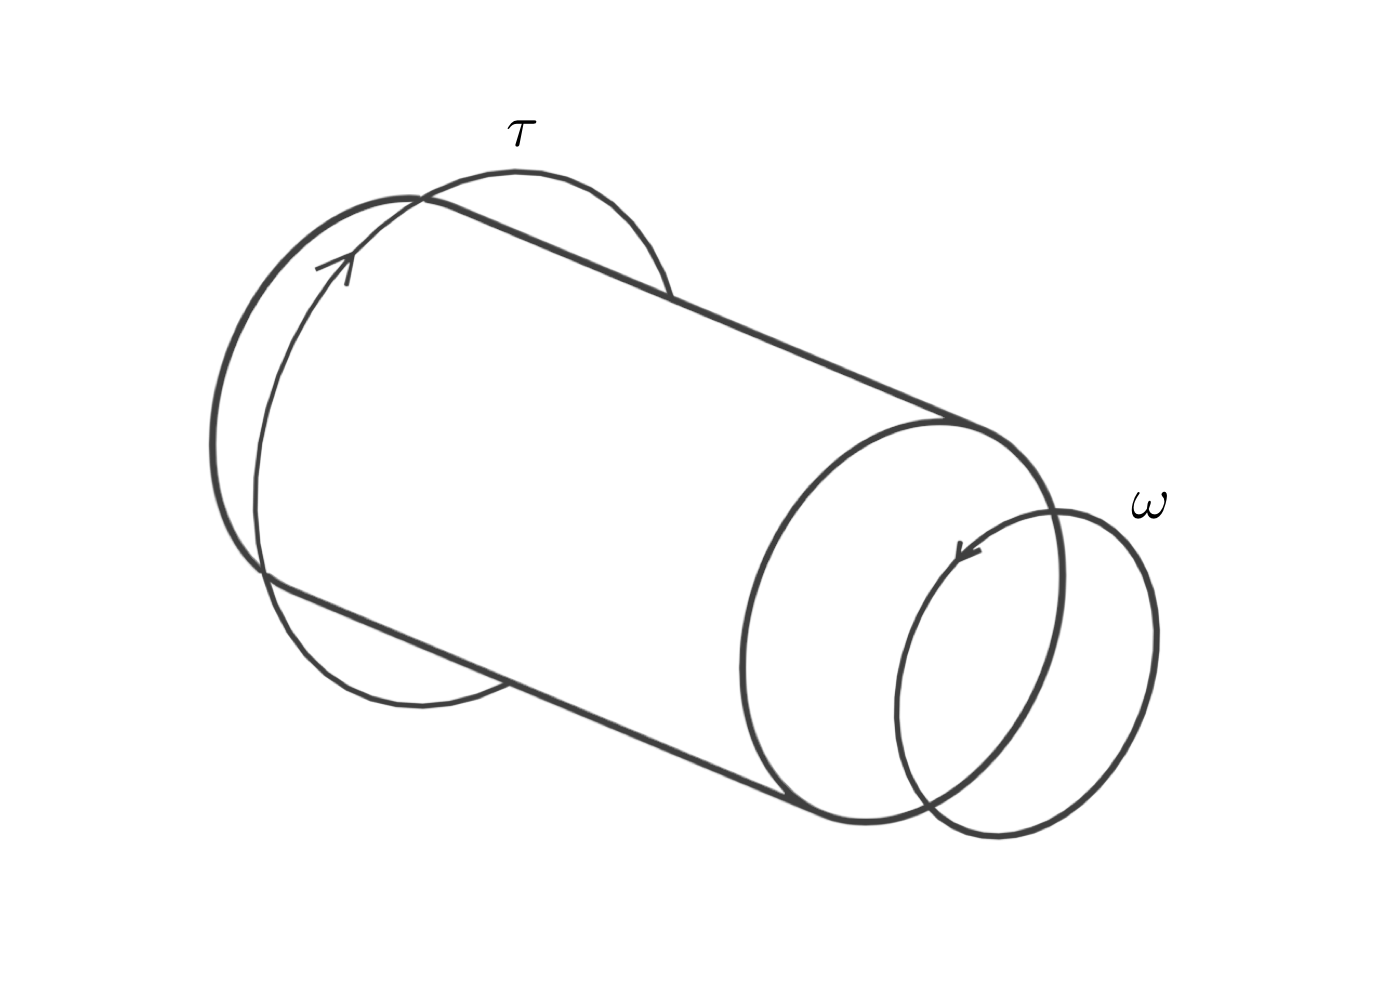
\includegraphics[width=\linewidth]{assets/20260725-1.png}
\end{minipage}
\end{center}

Assume the rotor has moment of inertia $I$ and no external torque acts on it.

\begin{questions}
  \item \textbf{A naive controller.}
        Dr.\ Wen first chooses the sensor
        \[
            S(\omega)=\omega-\omega_0 ,
        \]
        where $\omega_0>0$ is a constant.  Using the control law above and Newton's Second Law in rotational form, show that for any constant voltage $U$, the rotor converges to a steady angular velocity, and determine the steady-state value.

  \item \textbf{The improved controller.}
        Dr.\ Wen replaces the sensor with
        \[
            S(\omega)=\ln\left(\frac{\omega}{\omega_0}\right).
        \]
        He claims that logarithms are more suitable for controlling multiplicative quantities.  Show that the motor converges again, and determine the steady-state relation between $\omega$ and $U$.
\end{questions}

\end{problem}

\begin{solution}{20260725}

\subsection*{Q1. A naive controller}

\begin{align*}
    \tau &= I \dot \omega & &\text{(Newton)} \\
    k E &= I \dot \omega & &\text{(response)} \\
    k(\alpha U - S(\omega)) &= I \dot \omega & &\text{(instantiate)} \\
    k(\alpha U - \omega + \omega_0) &= I \dot \omega & &\text{(naive sensor)} \\
    \int \frac{\mathrm d \omega}{\alpha U + \omega_0 - \omega} &= \int \frac{k}{I}\;\mathrm d t & &\text{(separate)} \\
    -\ln|\alpha U + \omega_0 - \omega| &= \frac{k}{I}t + C & &\text{(integrate)} \\
    \omega(t) &= \alpha U + \omega_0 - C'e^{-kt/I} & &\text{(solve)}
\end{align*}
Taking the limit,
\[
    \omega_{\mathrm{ss}} = \lim_{t\to\infty}\omega(t) = \boxed{\alpha U + \omega_0}.
\]

\subsection*{Q2. The improved controller}

Instantiate the control law:
\[
    I \dot \omega = k\!\left(\alpha U - \ln\frac{\omega}{\omega_0}\right).
\]
At steady state $\dot\omega=0$, so
\[
    k\!\left(\alpha U - \ln\frac{\omega_{\mathrm{ss}}}{\omega_0}\right) = 0
    \;\Longrightarrow\;
    \ln\frac{\omega_{\mathrm{ss}}}{\omega_0} = \alpha U
    \;\Longrightarrow\;
    \omega_{\mathrm{ss}} = \omega_0 e^{\alpha U}.
\]
Convergence: rewrite the dynamics as
\[
    \dot\omega = \frac{k}{I}\!\left(\alpha U - \ln\frac{\omega}{\omega_0}\right).
\]
If $\omega>\omega_{\mathrm{ss}}$ then $\ln(\omega/\omega_0)>\alpha U$, so $\dot\omega<0$ (decelerates).  If $\omega<\omega_{\mathrm{ss}}$ then $\ln(\omega/\omega_0)<\alpha U$, so $\dot\omega>0$ (accelerates).  In both cases the rotor is driven toward $\omega_{\mathrm{ss}}$, hence
\[
    \boxed{\lim_{t\to\infty}\omega(t) = \omega_0 e^{\alpha U}}.
\]

\end{solution}

\input qpd-end

\input qpd-bootstrap

\begin{problem}{20260731}
  \meta{name}{Swing Dynamics}
  \meta{setter}{Jason Zhang}
  \meta{score}{10}
  \meta{topic}{mechanics}
  \meta{difficulty}{5}
  \meta{tags}{mechanics, pendulum, circular motion, energy, centripetal force}

A physics study group builds a small model of a swing.  A point mass $M$ hangs from a fixed pivot on a light string of length $L$.  Let $\theta$ be the angle the swing makes with the downward vertical.

At $t = 0$ the swing is at $\theta = 0$, but the mass has a velocity of magnitude $v_0$ directed normal to the string.  At some later time $t'$, the tension in the string returns to zero.

\begin{assumptions}
  \item The string is massless and inextensible, of length $L$.
  \item The pivot is fixed; the only force besides tension is gravity $g$.
  \item The mass is a point particle; air resistance is negligible.
\end{assumptions}

\begin{questions}
  \item \textbf{Over the horizontal.}
        Derive the minimum $v_0$ such that at $t = t'$, $\theta > \pi/2$ (the swing has passed the horizontal).

  \item \textbf{Over the top.}
        Derive the minimum $v_0$ such that at $t = t'$, $\theta > \pi$ (the swing has passed the vertical).

  \item \textbf{The point of no return.}
        Find the minimum angle $\theta^{*}$ with the following property: if the swing reaches $\theta = \theta^{*}$ with the string still taut, then the tension is positive at every angle beyond $\theta^{*}$.  (In other words, $\theta^{*}$ is the point of no return — once passed with the string taut, the swing is guaranteed to remain taut for the rest of the revolution.)
\end{questions}

\end{problem}

\begin{solution}{20260731}

Let $\theta$ be measured from the downward vertical.  The radial (outward) equation of motion is
\[
  T - Mg\cos\theta = -\frac{Mv^{2}}{L}
  \qquad\Longrightarrow\qquad
  T = M\frac{v^{2}}{L} + Mg\cos\theta,
\]
where $T \ge 0$ as long as the string is taut.  Conservation of energy gives
\[
  \tfrac12 M v^{2} + MgL(1-\cos\theta) = \tfrac12 M v_{0}^{2}
  \qquad\Longrightarrow\qquad
  v^{2} = v_{0}^{2} - 2gL(1-\cos\theta).
\]

\subsection*{Q1. Over the horizontal}

The string goes slack when $T = 0$:
\[
  \frac{v^{2}}{L} + g\cos\theta = 0
  \qquad\Longrightarrow\qquad
  v^{2} = -gL\cos\theta .
\]
Combining with energy,
\[
  -gL\cos\theta = v_{0}^{2} - 2gL(1-\cos\theta)
  \;\Longrightarrow\;
  v_{0}^{2} = gL(2 - 3\cos\theta).
\]
The slack angle $\theta'$ therefore satisfies $\cos\theta' = (2 - v_{0}^{2}/gL)/3$.  The condition $\theta' > \pi/2$ means $\cos\theta' < 0$, i.e.\ $v_{0}^{2} > 2gL$.  Hence
\[
  \boxed{v_{0,\min} = \sqrt{2gL}}.
\]

\subsection*{Q2. Over the top}

The condition $\theta' > \pi$ means $\cos\theta' < -1$ requires $v_{0}^{2} > 5gL$, so the boundary is $\theta' = \pi$, i.e.\ $\cos\theta' = -1$.  Then
\[
  v_{0}^{2} = gL(2 + 3) = 5gL
  \;\Longrightarrow\;
  \boxed{v_{0,\min} = \sqrt{5gL}}.
\]
At this speed the string goes slack exactly at the top, $\theta' = \pi$.

\subsection*{Q3. The point of no return}

Substituting the energy relation $v^{2} = v_{0}^{2} - 2gL(1-\cos\theta)$ into the tension gives
\[
  T(\theta) = M\frac{v^{2}}{L} + Mg\cos\theta
            = \frac{M}{L}\,v_{0}^{2} + Mg\bigl(3\cos\theta - 2\bigr).
\]
Since $\cos\theta$ is minimised at $\theta = \pi$, the tension is minimised at the top:
\[
  T_{\min} = T(\pi) = \frac{M}{L}\bigl(v_{0}^{2} - 5gL\bigr).
\]

Therefore, if the string is still taut at $\theta = \pi$ (so $T(\pi) > 0$), then $T(\theta) \ge T(\pi) > 0$ for every $\theta$, and in particular for every $\theta > \pi$.  So $\theta^{*} = \pi$ has the required property.

It is also the \emph{minimum}: for any $\theta^{*} < \pi$, choose a trajectory whose slack angle satisfies $\theta^{*} < \theta' < \pi$ (such trajectories exist, from Q1 with $\cos\theta' = (2 - v_{0}^{2}/gL)/3$).  Then $T(\theta^{*}) > 0$ yet $T(\theta') = 0$, so the property fails.  Hence no $\theta^{*} < \pi$ works, and
\[
  \boxed{\theta^{*} = \pi}.
\]
Equivalently: the string remains taut for the whole revolution precisely when $v_{0}^{2} \ge 5gL$, and the top is the last point at which it can first go slack.

\end{solution}

\input qpd-end

\input qpd-bootstrap

\begin{problem}{20260803}
  \meta{name}{The Trolley Problem}
  \meta{setter}{Andy He}
  \meta{score}{6}
  \meta{topic}{mechanics}
  \meta{difficulty}{2}
  \meta{tags}{mechanics, rotation, rolling, energy}

Today, SM-senior 黄瑞宣 was kidnapped by the evil Professor 孙笑川. The wicked Emperor has decided to make our great SM-senior 黄瑞宣 solve a problem that has long troubled humanity --- and, in doing so, to steal 李文亚's Nobel Prize. After weighing many awards, Professor 孙笑川 concluded that only the Nobel Prize in Physics could suppress 李文亚's white-body biology theory, so he resolved to have 黄瑞宣 solve a physics problem that has baffled all of humankind: the Trolley Problem. 黄瑞宣 had to choose between securing a pentakill for the ace elite and completing an online solo kill. Under Professor 孙笑川's coercion, and with the weight of past memories flooding back, 黄瑞宣 transformed on the spot into the Identity V character 破轮 (whose appearance is shown below).

\begin{center}
  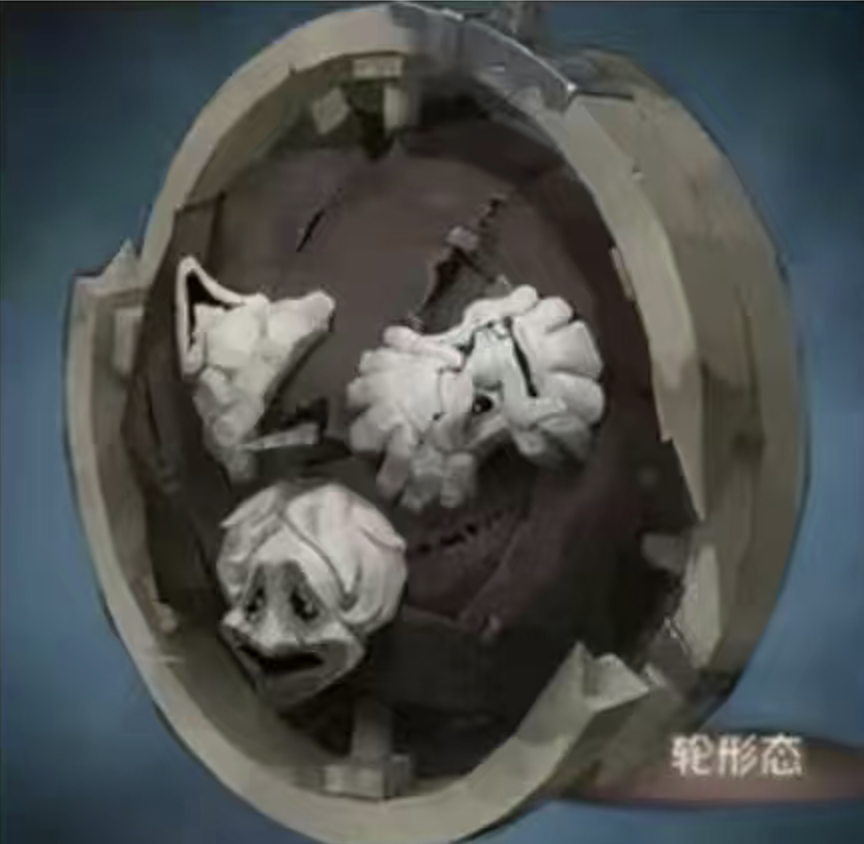
\includegraphics[width=0.45\linewidth]{assets/20260803-1.png}
\end{center}

…and crushed Professor 孙笑川 to death, bringing his sinful life to an end.

Treat Professor 孙笑川 as a hemisphere of radius $r$ lying on a plane. 黄瑞宣, having become 破轮, has radius $R$, mass $M$, and moment of inertia $I = \tfrac12 M R^{2}$, and has speed $v$ at the instant he crushes into Professor 孙笑川.

\begin{questions}
  \item Find the kinetic energy lost in rolling over Professor 孙笑川.
  \item Find the minimum initial speed $v$ for 黄瑞宣 to just barely roll over Professor 孙笑川.
\end{questions}

\end{problem}

\begin{solution}{20260803}

破轮 is a uniform disk, so its moment of inertia is $I = \tfrac12 M R^{2}$. When rolling without slipping on the ground, the total kinetic energy is the sum of translational and rotational parts:
\[
E_k = \tfrac12 M v^{2} + \tfrac12 I \omega^{2}
    = \tfrac12 M v^{2} + \tfrac12 \cdot \tfrac12 M R^{2}\!\left(\frac{v}{R}\right)^{2}
    = \tfrac34 M v^{2}.
\]

\textbf{Q1. Kinetic energy lost.} As 破轮 rolls from the ground (centre of mass at height $R$) up to the top of the hemisphere, its centre of mass rises to $R+r$, an increase of $\Delta h = r$. For ideal rolling without slipping there is no dissipation, so the kinetic energy lost is entirely converted into gravitational potential energy:
\[
\boxed{\Delta E_k = M g r}.
\]

\textbf{Q2. Minimum initial speed.} To \emph{just barely} roll over Professor 孙笑川, 破轮 arrives at the top of the hemisphere with zero kinetic energy. By conservation of mechanical energy,
\[
\tfrac34 M v_{\min}^{2} = M g r
\;\Longrightarrow\;
\boxed{v_{\min} = \sqrt{\tfrac{4}{3} g r}}.
\]

\end{solution}

\input qpd-end

\input qpd-bootstrap

\begin{problem}{20260804}
  \meta{name}{Plasma Cannon Launcher}
  \meta{setter}{Elton Liu}
  \meta{score}{13}
  \meta{status}{err}
  \meta{topic}{Mechanics}
  \meta{difficulty}{5}
  \meta{tags}{mechanics, rotation, projectile motion, energy}

Kai'Sa, the Daughter of the Void, fires plasma bolts from a device that can be modelled as an \emph{elastic rotating launcher}.  While charging a shot, Kai'Sa spins up a lightweight rigid launch arm of length $L$ (the arm's own mass is negligible); a plasma bolt of mass $m$ is fixed to the arm's tip.

During the charging phase the arm rotates counter-clockwise about a fixed pivot, starting from rest at the horizontal.  A variable external torque turns the arm against a torsional ``Hextech'' elastic structure, which produces a restoring torque
\[
  \tau = -k\theta ,
\]
where $\theta$ is the arm's angle from the horizontal.  When the arm reaches a maximum angle $\theta_{0}$, the bolt is released and flies off along the tangent, undergoing projectile motion under gravity $g$.  Air resistance, friction, the arm's mass, and all energy losses are neglected.

Given quantities: $m$, $L$, $k$, $\theta_{0}$, $g$.

\begin{assumptions}
  \item The arm is rigid and massless; the bolt is a point particle.
  \item The torsional spring obeys the linear law $\tau = -k\theta$.
  \item During charging, gravity's torque on the bolt is neglected (it is reintroduced only in Q5).
\end{assumptions}

\begin{questions}
  \item \textbf{Work in the charging phase.}
        Find the total work done by the external torque in charging the arm from $\theta = 0$ to $\theta = \theta_{0}$ against the torsional spring.

  \item \textbf{Rotational energy and angular speed.}
        At the instant of release, find
        \begin{enumerate}[label=\roman*.]
          \item the system's angular speed $\omega$;
          \item the bolt's instantaneous speed $v$;
          \item the bolt's instantaneous centripetal acceleration $a_c$.
        \end{enumerate}

  \item \textbf{Angular momentum: conserved or not?}
        A student claims: ``from the charging rotation through the instant of release, the system's angular momentum about the pivot is conserved.''  Judge whether this is right or wrong, and give a rigorous physical argument using torque and the angular-momentum theorem.

  \item \textbf{Projectile motion and mechanical energy.}
        The launch point is at height $H$, and the launch angle is $\theta_{0}$ (the velocity points along the tangent, at angle $\theta_{0}$ above the horizontal).  The bolt flies off and lands on the ground at height $0$.
        \begin{enumerate}[label=\roman*.]
          \item Using conservation of mechanical energy, write an expression for the landing speed $v_f$ (no need to work out the kinematics).
          \item If $\theta_{0}$ is very small (small-angle approximation), explain briefly how the horizontal range changes as $\theta_{0}$ increases, and give the physical reason.
        \end{enumerate}

  \item \textbf{Model extension: critical equilibrium.}
        Now include the torque that gravity exerts on the bolt.  Find the equilibrium angle position(s) $\theta$ at which the bolt can remain in static equilibrium (net torque zero).
\end{questions}

\end{problem}

\begin{solution}{20260804}

\subsection*{Q1. Work in the charging phase}

The external torque must overcome the restoring torque $-\k\theta$ at every instant, so the work it does is
\[
  W = \int_{0}^{\theta_{0}} k\theta \,\dd\theta
    = \boxed{\tfrac{1}{2}k\theta_{0}^{2}}.
\]

\subsection*{Q2. Rotational energy and angular speed}

All the work done in charging is stored in the spring and, at release, converted to the bolt's rotational kinetic energy.  The arm is massless, so the moment of inertia about the pivot is $I = mL^{2}$:
\[
  \tfrac{1}{2}k\theta_{0}^{2} = \tfrac{1}{2}I\omega^{2}
  = \tfrac{1}{2}mL^{2}\omega^{2}.
\]

\begin{enumerate}[label=\roman*.]
  \item $\displaystyle \omega = \theta_{0}\sqrt{\frac{k}{mL^{2}}} = \boxed{\frac{\theta_{0}}{L}\sqrt{\frac{k}{m}}}$.
  \item $\displaystyle v = \omega L = \boxed{\theta_{0}\sqrt{\frac{k}{m}}}$.
  \item $\displaystyle a_c = \omega^{2}L = \boxed{\frac{\theta_{0}^{2}k}{mL}}$.
\end{enumerate}

\subsection*{Q3. Angular momentum: conserved or not?}

\textbf{Wrong.}  The angular-momentum theorem states $\dfrac{\dd L}{\dd t} = \tau_{\text{net}}$, where $\tau_{\text{net}}$ is the net external torque about the pivot.  During charging the torsional spring exerts a nonzero torque $-\k\theta$ on the arm, and this torque is not balanced by anything --- it is precisely the external torque being worked against.  Since $\tau_{\text{net}} \ne 0$, the angular momentum is \emph{not} conserved.  (After release, gravity also exerts a moment about the original pivot on the freely flying bolt, further changing its angular momentum.)

\subsection*{Q4. Projectile motion and mechanical energy}

\begin{enumerate}[label=\roman*.]
  \item After release the only force doing work is gravity, so mechanical energy is conserved:
  \[
    \tfrac{1}{2}mv_{f}^{2} = \tfrac{1}{2}mv^{2} + mgH
    \;\Longrightarrow\;
    \boxed{v_{f} = \sqrt{v^{2} + 2gH}}.
  \]
  Substituting $v = \theta_{0}\sqrt{k/m}$ gives $v_{f} = \sqrt{\dfrac{\theta_{0}^{2}k}{m} + 2gH}$.

  \item For small $\theta_{0}$, the horizontal range \emph{increases} as $\theta_{0}$ increases.  Physically, the horizontal velocity $v\cos\theta_{0}$ barely changes (it is $\approx v$), while the upward velocity $v\sin\theta_{0}$ grows roughly linearly with $\theta_{0}$; a larger upward velocity means a longer time of flight, which dominates, so the bolt travels farther.  (The exact range from height $H$ grows as $\dfrac{v^{2}}{g}\theta_{0} + v\sqrt{2H/g}$ for small $\theta_{0}$.)
\end{enumerate}

\subsection*{Q5. Model extension: critical equilibrium}

With the bolt at the tip, gravity exerts a torque about the pivot equal to $-mgL\cos\theta$ (the lever arm is the horizontal distance $L\cos\theta$ from the pivot to the bolt).  The spring exerts $-k\theta$, so static equilibrium requires
\[
  -k\theta - mgL\cos\theta = 0
  \;\Longrightarrow\;
  \boxed{k\theta + mgL\cos\theta = 0}.
\]
For $\theta > 0$ both torques point the same way (back toward horizontal), so there is no equilibrium above horizontal.  The balance is possible only \emph{below} horizontal, where the spring pulls upward and gravity pulls downward; there the equilibrium angle solves the transcendental equation
\[
  \boxed{\theta = -\frac{mgL}{k}\cos\theta}.
\]

\end{solution}

\input qpd-end

\input qpd-bootstrap

\begin{problem}{20260808}
  \meta{name}{Binary Star System}
  \meta{setter}{Sophie Chen}
  \meta{score}{12}
  \meta{topic}{gravitation}
  \meta{difficulty}{4}
  \meta{tags}{gravitation, orbital motion, Kepler}

A binary star system consists of two stars orbiting their common centre of mass.  Star A has mass $M_A = 4\times10^{30}\,\mathrm{kg}$ and Star B has mass $M_B = 1\times10^{30}\,\mathrm{kg}$.  The straight-line distance between the two stars is $D = 5.0\times10^{12}\,\mathrm{m}$, and the gravitational constant is $G = 6.67\times10^{-11}\,\mathrm{N\,m^{2}\,kg^{-2}}$.  The two stars orbit their shared centre of mass in perfect uniform circular motion.

\begin{assumptions}
  \item The stars are point masses; only their mutual gravitational attraction acts.
  \item The orbits are circular and coplanar, about the common centre of mass.
\end{assumptions}

\begin{questions}
  \item \textbf{Equal and Opposite Forces.}
        Compare the magnitude of the gravitational pull that Star A exerts on Star B with the pull that Star B exerts on Star A.  State whether they are larger, smaller, or equal, and name the physics law that supports your conclusion.

  \item \textbf{The Zero-Force Point.}
        Along the line connecting Star A and Star B there is a unique point where the total gravitational force on a tiny test mass $m$ placed at that position cancels out to zero.
        \begin{enumerate}[label=\arabic*.]
          \item Let $x$ be the distance from Star A to this zero-force point.  Write the gravitational force-balance equation for the test mass.
          \item Solve numerically to calculate the value of $x$.
        \end{enumerate}

  \item \textbf{Orbital Period.}
        The zero-force point from part (b) is \emph{not} the system's centre of mass.  Both stars revolve around their common centre of mass with identical period $T$.
        \begin{enumerate}[label=\arabic*.]
          \item Write the equation equating the mutual gravitational force to the centripetal force for Star A.
          \item Write the matching force equation for Star B.
          \item Combine the two equations to derive the modified Kepler's Third Law for binary stars, then substitute the given numbers to solve for the orbital period $T$ of the system.
        \end{enumerate}

  \item \textbf{Orbital Speeds.}
        Derive and write a single equality relating $M_A$, $M_B$, $v_A$, and $v_B$.  No numerical calculation is needed here.
\end{questions}

\end{problem}

\begin{solution}{20260808}

\subsection*{Q1. Equal and Opposite Forces}

By Newton's Third Law the two pulls are equal and opposite: $\abs{\arr{F}_{A\to B}} = \abs{\arr{F}_{B\to A}}$.

\subsection*{Q2. The Zero-Force Point}

\textbf{(1)}  On the line AB the forces on $m$ are collinear and opposite, so they cancel when
\[
\frac{G M_A m}{x^{2}} = \frac{G M_B m}{(D-x)^{2}}
\;\Longrightarrow\;
\frac{M_A}{x^{2}} = \frac{M_B}{(D-x)^{2}}.
\]

\textbf{(2)}  Taking square roots and solving:
\[
x = D\,\frac{\sqrt{M_A}}{\sqrt{M_A}+\sqrt{M_B}}
  = (5.0\times10^{12})\,\frac{2\times10^{15}}{3\times10^{15}}
  = \boxed{3.3\times10^{12}\ \mathrm{m}}.
\]

\subsection*{Q3. Orbital Period}

Let $r_A + r_B = D$ be the orbital radii about the common centre of mass, with $\omega = 2\pi/T$.  Equating the mutual force to the centripetal force for each star,
\[
\frac{G M_A M_B}{D^{2}} = M_A\omega^{2} r_A = M_B\omega^{2} r_B.
\]
With $M_A r_A = M_B r_B$ and $r_A+r_B=D$, we get $r_A = \dfrac{M_B D}{M_A+M_B}$; substituting and using $\omega = 2\pi/T$ gives the modified Kepler's Third Law:
\[
\boxed{T^{2} = \frac{4\pi^{2}D^{3}}{G(M_A+M_B)}}.
\]
Numerically, with $M_A+M_B = 5.0\times10^{30}\,\mathrm{kg}$:
\[
T = 2\pi\sqrt{\frac{(5.0\times10^{12})^{3}}{(6.67\times10^{-11})(5.0\times10^{30})}}
  = \boxed{3.8\times10^{9}\ \mathrm{s}} \approx 122\ \text{yr}.
\]

\subsection*{Q4. Orbital Speeds}

Same angular speed means $v_A/v_B = r_A/r_B = M_B/M_A$, hence
\[
\boxed{M_A v_A = M_B v_B}.
\]

\end{solution}

\input qpd-end

\input qpd-bootstrap

\begin{problem}{20260811}
  \meta{name}{Vector Triangles and Their Simple Applications}
  \meta{setter}{Ryan Huang, Sophie Chen}
  \meta{score}{7}
  \meta{topic}{Mechanics}
  \meta{difficulty}{3}
  \meta{tags}{mechanics, kinematics, projectile motion}

    
\emph{The vector triangle is a practical and common tool in physics, yet it barely appears in AP examinations.  What follows is a brief introduction, a worked example, and a set of problems for the reader to explore.}

\subsection*{Concept and Example}

Consider the following scenario.  A point mass $m$ is launched from the ground at an angle $\theta$; its initial velocity $\arr{v}_{0}$ is the leftmost vector in Figure~1.  Throughout the motion a constant downward acceleration of magnitude $g$ acts on the body --- that is the vector on the right of the $+$ sign in the figure.  At landing the velocity is the vector to the right of the $=$ sign.  The whole evolution can therefore be synthesised into the triangle shown on the right.

\begin{center}
    \begin{minipage}{0.85\textwidth}
    \centering
    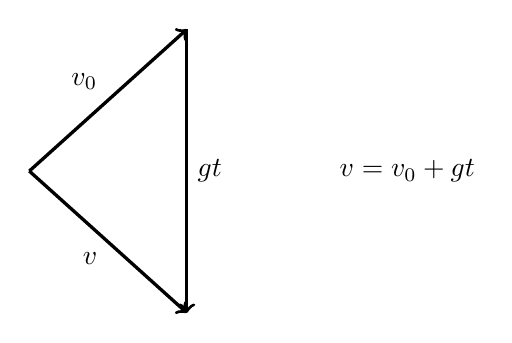
\begin{tikzpicture}[scale=1]
      % -- v0 (launch) --
      \draw[->,very thick] (0,0) -- (2,1.8)
        node[midway,above left] {$\arr{v}_{0}$};
      % -- gt (straight down from tip of v0) --
      \draw[->,very thick] (2,1.8) -- (2,-1.8)
        node[midway,right] {$\arr{g}t$};
      % -- v (final, tip-to-tail from origin) --
      \draw[->,very thick] (0,0) -- (2,-1.8)
        node[midway,below left] {$\arr{v}$};
      % -- label --
    
      \node at (4.8,0) {$\arr{v} = \arr{v}_{0} + \arr{g}t$};
    \end{tikzpicture}
    \par\smallskip
    \textit{Fig.~1 --- The vector triangle for ground-to-ground projectile motion.  $\arr{v}_{0}$ and $\arr{g}t$ have fixed directions; $\arr{v}$ and the flight time $t$ vary with $\theta$.}
    \end{minipage}
\end{center}

This construction leads to a classic question: at what angle $\theta$ must one launch the mass to maximise the horizontal range?  Intuition (and elementary kinematics plus trigonometry) gives $45^{\circ}$.  Here we offer a different approach --- using the \emph{area} of the vector triangle.

Integrating velocity gives displacement, so let us examine the area of the triangle formed by $\arr{v}_{0}$, $\arr{g}t$, and $\arr{v}$.  A short calculation (left to the reader in Q1 below) shows that
\[
  S = \tfrac{1}{2}\,gx, \tag{3}
\]
where $x$ is the horizontal range.  Notice that the area depends \emph{only} on $x$; once we express $S$ in terms of the launch parameters, maximising $x$ reduces to maximising the area of a triangle with two sides of fixed length.

Indeed, in our triangle one side ($\arr{g}t$) changes with the flight time, but another view fixes $\arr{v}_{0}$ and varies the angle $\alpha$ between $\arr{v}_{0}$ and $\arr{v}$.  A second calculation (Q2) yields
\[
  S = \tfrac{1}{2}\,v_{0}^{2}\sin 2\theta
    = -\tfrac{1}{2}\,v_{0}^{2}\sin 2\alpha. \tag{4}
\]
From either expression the maximum occurs at $\theta = 45^{\circ}$, recovering the familiar result through a purely geometric route.

\newpage

\subsection*{Problems}

The following exercises walk you through the derivation sketched above and extend the idea to a slightly more general setting.

\begin{assumptions}
  \item Flat, level ground; uniform gravity $\arr{g} = -g\,\hat{\mathbf{y}}$; no air resistance.
  \item The vector triangle is formed by $\arr{v}_{0}$, $\arr{g}t$, and $\arr{v}$ at the instant of landing ($y = 0$).
  \item In Q3 the launch point is elevated: $y(0) = h$, $y(t_{\text{land}}) = 0$.
\end{assumptions}

\begin{questions}
  \item \textbf{Area in terms of range.}
        Consider the same scenario as the example above (ground-to-ground).
        Prove that the area of the vector triangle is
        \[
          S = \tfrac{1}{2}\,gx,
        \]
        where $x$ is the horizontal range of the projectile.

  \item \textbf{Area in angular form.}
        For the same scenario, show that the area can also be written as
        \[
          S = \tfrac{1}{2}\,v_{0}^{2}\sin 2\theta
            = -\tfrac{1}{2}\,v_{0}^{2}\sin 2\alpha,
        \]
        where $\alpha$ is the angle between $\arr{v}_{0}$ and $\arr{v}$.  Use either expression to confirm that the range is maximised at $\theta = 45^{\circ}$.

  \item \textbf{Non-zero launch height.}
        Now the mass is launched from $y = h > 0$ and lands at $y = 0$ (all else unchanged).  Determine the angle $\theta$ that maximises the horizontal distance $L$.  No resistance of any kind.

        \textit{Hint:} the vector-triangle idea generalizes --- think about what changes when the launch and landing heights differ.
\end{questions}

\end{problem}

\begin{solution}{20260811}

\subsection*{Q1. Area in terms of range}

Let the flight time be $t$.  Resolving the initial velocity,
\[
\arr{v}_{0} = (v_{0}\cos\theta, v_{0}\sin\theta),
\qquad
\arr{g}t = (0, -gt).
\]

The cross-product magnitude of any two sides of the triangle gives (twice) its area.  Choosing $\arr{v}_{0}$ and $\arr{g}t$,
\[
2S = \abs{\arr{v}_{0} \times (\arr{g}t)}
    = \abs{(v_{0}\cos\theta)(-gt) - (v_{0}\sin\theta)(0)}
    = gtv_{0}\cos\theta.
\]

Since $x = v_{0}\cos\theta \cdot t$ is precisely the horizontal range, hence
\[
\boxed{S = \tfrac{1}{2}gx}.
\]

\subsection*{Q2. Area in angular form}

For ground-to-ground motion, the vertical displacement is zero:

\[
0 = v_{0}\sin\theta \cdot t - \tfrac 1 2 gt^{2}
\;\Longrightarrow\;
t = \frac{2v_{0}\sin\theta}{g}.
\]

Substituting into the area formula of Q1,
\[
S = \tfrac{1}{2}\,g\,(v_{0}\cos\theta)\,
      \frac{2v_{0}\sin\theta}{g}
  = \boxed{\tfrac{1}{2}\,v_{0}^{2}\sin 2\theta}.
\]

Now consider the same triangle but with the two sides $\arr{v}_{0}$ and
$\arr{v}$ meeting at the origin.  For ground-to-ground motion, energy
conservation gives $\abs{\arr{v}} = \abs{\arr{v}_{0}} = v_{0}$.  The
(signed) area of the triangle is
\[
S = \tfrac{1}{2}\,\abs{\arr{v}_{0}}\,\abs{\arr{v}}\,\sin\alpha
  = \tfrac{1}{2}\,v_{0}^{2}\sin\alpha,
\]
where $\alpha$ is the interior angle at the origin, taken from $\arr{v}_{0}$
to $\arr{v}$.  At landing $\arr{v} = (v_{0}\cos\theta,\,-v_{0}\sin\theta)$,
so $\alpha = -2\theta$ (the velocity has rotated clockwise by $2\theta$).
Hence
\[
\sin\alpha = \sin(-2\theta) = -\sin 2\theta,
\qquad
S = -\tfrac{1}{2}\,v_{0}^{2}\sin\alpha.
\]

The two forms are therefore equivalent:  $\boxed{S
= \tfrac{1}{2}v_{0}^{2}\sin 2\theta
= -\tfrac{1}{2}v_{0}^{2}\sin\alpha}$.

The maximum of $S$ --- and therefore of $x$ --- occurs when $\sin 2\theta = 1$,
i.e.\ $\boxed{\theta = 45^{\circ}}$, recovering the familiar result through a
purely geometric route.

\subsection*{Q3.  Non-zero launch height}

The mass is launched from $y = h > 0$ and lands at $y = 0$.  The flight time
satisfies
\[
0 = h + v_{0}\sin\theta \cdot t - \tfrac{1}{2}gt^{2},
\]
giving
\[
t(\theta) = \frac{v_{0}\sin\theta
                + \sqrt{v_{0}^{2}\sin^{2}\theta + 2gh}}{g}.
\]

The horizontal range is $L(\theta) = v_{0}\cos\theta \cdot t(\theta)$.

To maximise $L$, set $\dd L/\dd\theta = 0$.  Writing $L$ explicitly and
differentiating (or, more elegantly, using the implicit relation
$L\tan\theta - gL^{2}/(2v_{0}^{2}\cos^{2}\theta) + h = 0$ obtained by
eliminating $t$), one finds
\[
\boxed{\sin^{2}\theta_{\text{opt}}
       = \frac{v_{0}^{2}}{2(v_{0}^{2} + gh)}}.
\]

Equivalently,
\[
\theta_{\text{opt}} = \arcsin\sqrt{\frac{v_{0}^{2}}{2(v_{0}^{2}+gh)}},
\qquad\text{or}\qquad
\tan\theta_{\text{opt}} = \frac{v_{0}}{\sqrt{v_{0}^{2} + 2gh}}.
\]

\medskip
\noindent\textit{Geometric note.}
From Q1, $S = \tfrac{1}{2}gL$ still holds.  Energy conservation gives
$\abs{\arr{v}}^{2} = v_{0}^{2} + 2gh$, so the two sides meeting at the origin
have \emph{fixed} lengths $v_{0}$ and $\sqrt{v_{0}^{2}+2gh}$.
The area $S = \tfrac{1}{2}v_{0}\abs{\arr{v}}\sin\varphi$ (where $\varphi$
is the angle between $\arr{v}_{0}$ and $\arr{v}$) is maximised when
$\varphi = 90^{\circ}$, i.e.\ when $\arr{v}_{0} \perp \arr{v}$.
Imposing orthogonality on the vector triangle yields the same optimal angle
as above, without calculus.

\end{solution}

\input qpd-end

\input qpd-bootstrap

\begin{problem}{20260813}
  \meta{name}{Tossing the Wok}
  \meta{setter}{Sean Li}
  \meta{score}{7}
  \meta{topic}{mechanics}
  \meta{difficulty}{4}
  \meta{tags}{mechanics, rotation, energy, kinematics, rigid body}
  \meta{open}{true}
\begin{assumptions}
\item The accelerations are prescribed kinematically --- think of them as constraints imposed by the pan, not as net forces acting on a free body. Do NOT add $g$ to the net acceleration when $t < t_0$.
\end{assumptions}
\begin{center}
\begin{minipage}[c]{0.55\textwidth}
Dr.\ Wen is learning to \emph{toss the wok} --- the classical technique of jerking a pan sharply to flip its contents.

Model the pancake $\Omega$ as a uniform rigid disk of radius $R$ and planar mass density $\rho$, initially lying in the $xy$-plane with its center of mass at the origin.

At $t = 0$, two constant accelerations are applied for $[0, t_0]$:
\begin{enumerate}
    \item Angular acceleration $\alpha$ about an in-plane axis through the
    center of mass (the ``flipping axis'').
    \item Linear acceleration $\arr{a}$ of the CM, vertical component $a$.
\end{enumerate}

At $t = t_0$ the forces cease.  An \textbf{$n$-toss} is \emph{successful} if at some $t' > t_0$ the pancake returns exactly to its original spatial region, and the rigid motion between the two configurations is a pure rotation by $n\pi$ about the flipping axis.

Dr.\ Wen cooks in vacuum. Do not consider air resistance.
\end{minipage}%
\hfill
\begin{minipage}[c]{0.42\textwidth}
\centering
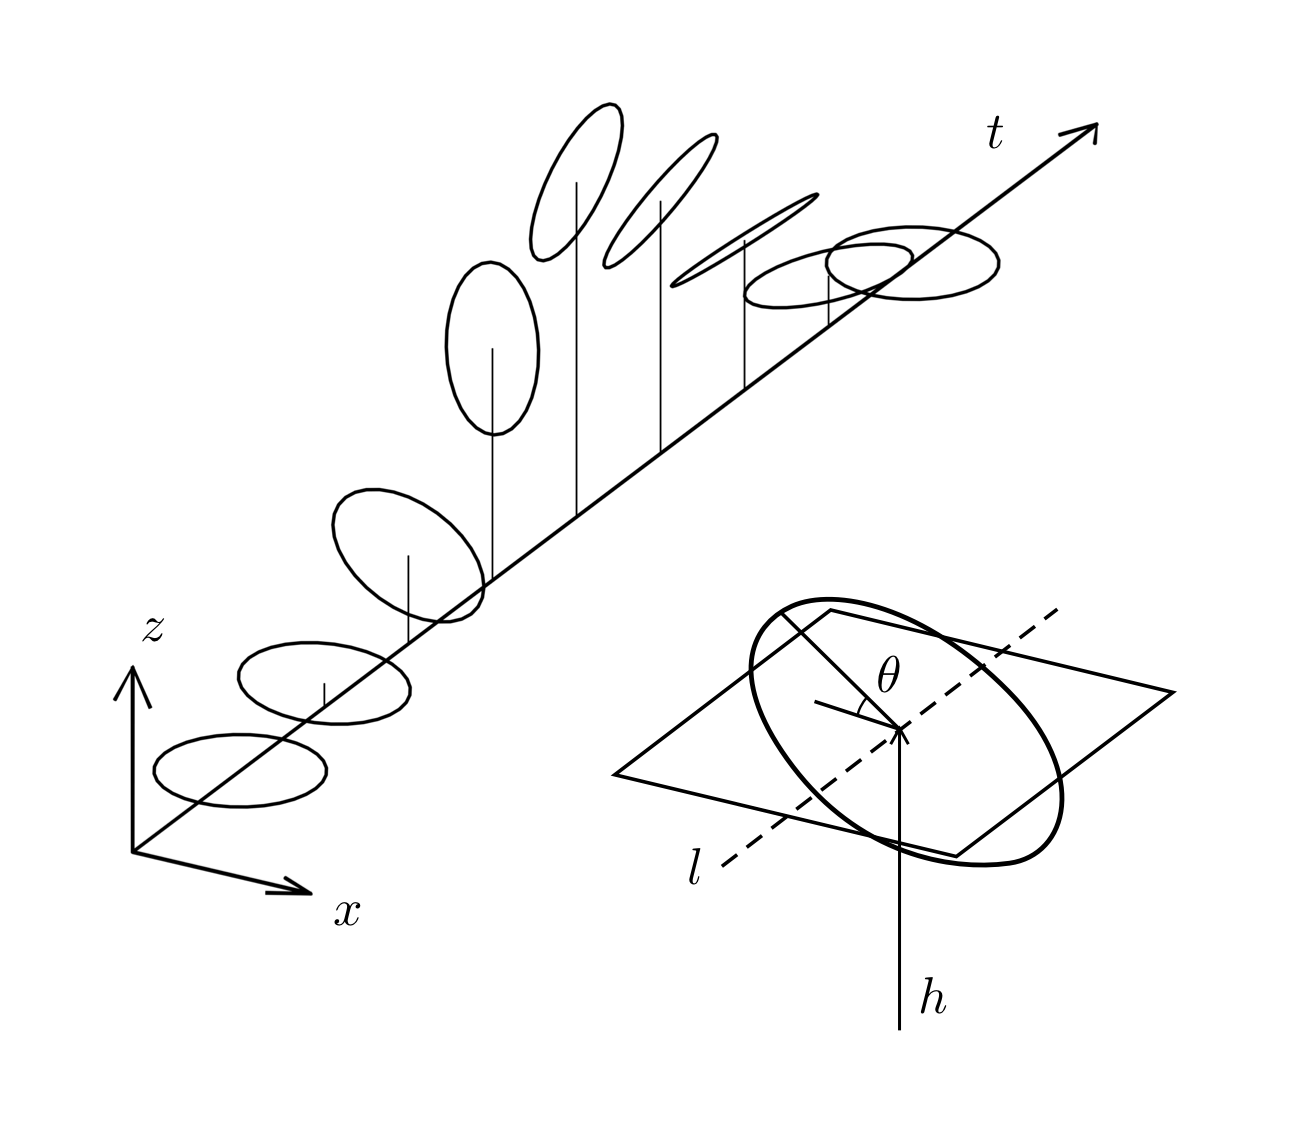
\includegraphics[width=\linewidth]{assets/20260812-1.png}
\captionof{figure}{The pancake at different $t$ during a $1$-toss.  $\theta$ is
the rotation about the flipping axis $\ell$ ($\ddot\theta=\alpha$ for $t<t_0$),
and $h$ the CM height ($\ddot h=a$ for $t<t_0$).}
\end{minipage}
\end{center}


\begin{questions}
    \item \textbf{Toss Constraint.}
    Formulate an equation that relates $n$, $\alpha$, $a$, and $t_0$ for any $n > 0$.

    \item \textbf{Toss Energy Ladder.}
    Derive the work $W$ done on the pancake as an expression containing $n$, $\alpha$, $a$ and other physical constants, and show that $W \propto n$.

    \item \textbf{Cracked Pancake.}

    \begin{center}
    \begin{minipage}[c]{0.52\textwidth}
    While tossing, Dr.\ Wen's pancake cracks exactly along the flipping axis, splitting it into two equal half-disks.  He hastily glues them back together with egg yolk, which can provide a total binding force of at most $F_y$ normal to the crack.

    During the forced phase ($t < t_0$), the rotation accelerates, creating an outward centrifugal tendency on each half-disk.  If the required centripetal force exceeds $F_y$, the halves separate and the toss is ruined. 

    Given $n$ (and the toss constraint from Q1), find the minimum $F_y$ as an expression of $n$, $a$, $\alpha$, $m$ and other physical constants needed to prevent splitting.
    \end{minipage}%
    \hfill
    \begin{minipage}[c]{0.42\textwidth}
    \centering
    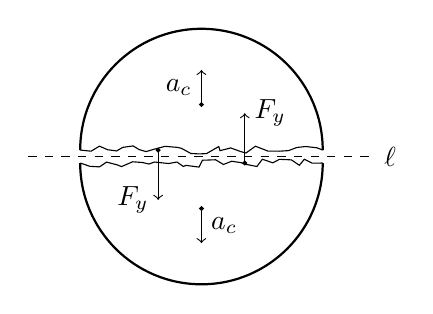
\begin{tikzpicture}[scale=1.1]
        % Upper half-disk
        \draw[thick] (-1.4,0.075) arc(180:0:1.4);
        \draw[decorate, decoration={random steps, segment length=3pt, amplitude=1.5pt}] (1.4,0.075) -- (-1.4,0.075);
        % Lower half-disk
        \draw[thick] (-1.4,-0.075) arc(180:360:1.4);
        \draw[decorate, decoration={random steps, segment length=3pt, amplitude=1.5pt}] (1.4,-0.075) -- (-1.4,-0.075);
        \draw[dashed] (-2.0,0) -- (2.0,0) node[right] {$\ell$};
        \filldraw (-0.5,0.075) circle (0.6pt);
        \draw[->] (-0.5,0.075) -- (-0.5,-0.5) node[at end,left] {$\arr{F}_y$};
        \filldraw (0.5,-0.075) circle (0.6pt);
        \draw[->] (0.5,-0.075) -- (0.5,0.5) node[at end,right] {$\arr{F}_y$};
        \filldraw (0,0.6) circle (0.6pt);
        \draw[->] (0,0.6) -- (0,1.0) node[midway,left] {$\arr{a}_c$};
        \filldraw (0,-0.6) circle (0.6pt);
        \draw[->] (0,-0.6) -- (0,-1.0) node[midway,right] {$\arr{a}_c$};
    \end{tikzpicture}
    \end{minipage}
    \end{center}
\end{questions}

\end{problem}

\begin{solution}{20260813}

Let $\mathbf q(t) = \langle h(t), \theta(t)\rangle$ with $h$ the CM vertical displacement and $\theta$ the rotation about the flipping axis.  The trajectory is piecewise-constant acceleration:
\[
\ddot{\mathbf q} =
\begin{cases}
\langle a, \alpha \rangle, & 0 \le t < t_0 \quad\text{(Forced)}\\[2pt]
\langle -g, 0 \rangle,      & t_0 \le t \le t' \quad\text{(Free fall)}
\end{cases}
\]
with $\mathbf q(0) = \dot{\mathbf q}(0) = \langle 0,0\rangle$ and $\mathbf q(t') = \langle 0, n\pi\rangle$.

\subsection*{Q1. Toss Constraint}

\textit{Phase 1} ($0 \le t < t_0$): constant acceleration, zero initial conditions.  Integrating twice:
\begin{align*}
\dot{\mathbf q}(t_0) &= t_0\langle a,\alpha\rangle,
& \mathbf q(t_0) &= \tfrac12 t_0^2\langle a,\alpha\rangle.
\end{align*}
Hence $h_0 \equiv h(t_0) = \tfrac12 a t_0^2$, $\dot h_0 \equiv \dot h(t_0) = a t_0$, $\theta_0 \equiv \theta(t_0) = \tfrac12 \alpha t_0^2$, $\dot\theta_0 \equiv \dot\theta(t_0) = \alpha t_0$.

\textit{Phase 2} ($t_0 \le t \le t'$): free motion under gravity (no torque).  Let $\Delta t = t' - t_0$.  Then
\begin{align*}
h(t') &= h_0 + \dot h_0\,\Delta t - \tfrac12 g(\Delta t)^2
      = \tfrac12 a t_0^2 + a t_0\Delta t - \tfrac12 g\Delta t^2, \\[4pt]
\theta(t') &= \theta_0 + \dot\theta_0\,\Delta t
           = \tfrac12 \alpha t_0^2 + \alpha t_0\Delta t.
\end{align*}

Success requires $h(t') = 0$ and $\theta(t') = n\pi$.  From $h(t') = 0$ (quadratic in $\Delta t$, positive root):
\[
\Delta t = \frac{t_0}{g}\Bigl(a + \sqrt{a(a+g)}\Bigr). \tag{1}
\]
From $\theta(t') = n\pi$:
\[
\Delta t = \frac{2\pi n - \alpha t_0^2}{2\alpha t_0}. \tag{2}
\]
Equating (1) and (2) gives the \textbf{toss constraint}:
\[
\boxed{\frac{\alpha t_0^2}{2g}\,\Bigl(2\sqrt{a(a+g)} + 2a + g\Bigr) = \pi n}
\qquad\text{or}\qquad
\boxed{t_0^2 = \frac{2\pi g n}{\alpha\bigl(2\sqrt{a(a+g)} + 2a + g\bigr)}}.
\]

\subsection*{Q2. Toss Energy Ladder}

The pancake is a uniform disk of radius $R$, mass $m = \pi R^2\rho$.  Its moment of inertia about the flipping axis (in-plane, through CM) is $I = \int_\Omega y^2\,\mathrm{d}m$.  In polar coordinates:
\begin{align*}
I &= \int_0^{2\pi}\!\int_0^R (r\sin\theta)^2 \rho\,r\,\mathrm{d}r\,\mathrm{d}\theta
  = \rho \int_0^{2\pi}\!\sin^2\theta\,\mathrm{d}\theta \int_0^R r^3\,\mathrm{d}r \\[4pt]
  &= \rho \cdot \pi \cdot \frac{R^4}{4}
  = \frac{1}{4} m R^2.
\end{align*}
Since the axis passes through CM, kinetic energy separates: $E(t) = m g h(t) + \tfrac12 m \dot h(t)^2 + \tfrac12 I \dot\theta(t)^2$.  At $t = 0$ all terms vanish ($E(0) = 0$).  The work done by the pan is $W = E(t_0)$:
\begin{align*}
W &= m g\!\left(\tfrac12 a t_0^2\right)
    + \tfrac12 m (a t_0)^2
    + \tfrac12\!\left(\tfrac14 m R^2\right)(\alpha t_0)^2 \\[4pt]
  &= \frac{m t_0^2}{8}\Bigl(R^2\alpha^2 + 4a^2 + 4a g\Bigr).
\end{align*}
Substituting $t_0^2$ from the toss constraint ($t_0^2 \propto n$):
\[
\boxed{W = \frac{\pi g m n}{4\alpha}\,
    \frac{R^2\alpha^2 + 4a^2 + 4a g}{2\sqrt{a(a+g)} + 2a + g}
    \;\propto\; n}.
\]

\subsection*{Q3. Cracked Pancake}

The crack splits the disk along the $x$-axis (the flipping axis) into upper ($y>0$) and lower ($y<0$) half-disks, each of mass $m/2$.

\emph{Center of mass of a uniform half-disk.}  By symmetry $\bar x = 0$.  For $\bar y$, integrate over the upper half-disk:
\[
\bar y = \frac{1}{m/2}\int_{\text{half}} y\,\mathrm{d}m
       = \frac{2}{m}\int_0^\pi\!\!\int_0^R (r\sin\theta)\,\rho\,r\,\mathrm{d}r\,\mathrm{d}\theta.
\]
With $m = \pi R^2\rho$:
\begin{align*}
\bar y &= \frac{2\rho}{\pi R^2\rho}
         \int_0^\pi \sin\theta\,\mathrm{d}\theta \int_0^R r^2\,\mathrm{d}r
       = \frac{2}{\pi R^2}\cdot \bigl[-\cos\theta\bigr]_0^\pi \cdot \frac{R^3}{3} \\[4pt]
       &= \frac{2}{\pi R^2}\cdot 2 \cdot \frac{R^3}{3}
       = \frac{4R}{3\pi}.
\end{align*}
Let $d = \bar y = 4R/(3\pi)$ be the CM distance from the flipping axis.

During the forced phase the upper half-disk's CM undergoes circular motion about the $x$-axis with $\omega(t) = \alpha t$.  The centripetal force required is
\[
F_{\text{cent}}(t) = \frac{m}{2}\,\omega(t)^2\,d
                   = \frac{2mR}{3\pi}\,\alpha^2 t^2.
\]
The egg yolk supplies this across the crack; the maximum occurs at $t = t_0$: $F_{\text{cent,max}} = \frac{2mR}{3\pi}\,\alpha^2 t_0^2$.

Using $t_0^2$ from the toss constraint (Q1):
\begin{align*}
F_{\text{cent,max}}
  &= \frac{2mR}{3\pi}\,\alpha^2\,
     \frac{2\pi g n}{\alpha\bigl(2\sqrt{a(a+g)} + 2a + g\bigr)} \\[4pt]
  &= \frac{4 R \alpha g m n}{3\bigl(2\sqrt{a(a+g)} + 2a + g\bigr)}.
\end{align*}

Therefore the egg yolk must satisfy
\[
\boxed{F_y \ge \frac{4R\alpha g m n}{3\bigl(2\sqrt{a(a+g)} + 2a + g\bigr)}}.
\]
The right-hand side is finite for any finite $\alpha$, $a$, $n$ --- a finite $F_y$ always suffices.  The required force scales linearly with both $n$ and $\alpha$: more flips or a more aggressive spin demand stronger glue.

\end{solution}

\input qpd-end
\end{document}
